\section{实验}
\label{sec:experiment}

这一章节将会利用上一章介绍的高斯混合模型的背景建模方法在视频序列图像上进行实验,并对其实现效果、实时性进行展示和分析。

首先,对手动实现的高斯混合模型、分别在 R、G、B 三个通道手动实现的高斯混合模型及调用的 OpenCV 高斯混合模型函数的实现效果进行对比。对于手动实现的高斯混合模型,分别设置参数 $K=4$,$\alpha = 0.005$,$T = 0.75$,初始 $\mu = 0$,$\sigma = 30$,$w = 0.1$。对于 OpenCV 高斯混合模型函数,设置输入参数和手动实现的训练图像数量相同, $\text{varThreshold}=100$。可视化结果(部分)如图 \ref{fig:result} 所示。

从图 \ref{fig:result} 可以看出,对于两种手动实现的方法而言,相比于在灰度图上对每个像素进行高斯混合模型建模,分别在 R、G、B 三个通道对每个像素进行建模获得的结果更加准确,表现在目标更加完整,作为前景的车辆空洞更少。但多通道的高斯混合模型建模方法也带来了更大的计算开销,约为前者的三倍。而调用的 OpenCV 高斯混合模型函数虽然其训练及测试速度较快,但其效果略差,一方面噪声较多且目标中存在大量空洞,另一方面即使传入了对阴影检测的参数,实际结果也仍有部分阴影被分为前景。三种实现方法的实时性如表 \ref{tab:measurement} 所示。

\begin{table}[!htbp]
\caption{不同实现方法的实时性比较}
\centering
\label{tab:measurement}
\setlength{\tabcolsep}{2mm}{
\begin{tabular}{c|c|c|c}
\hline
& 手动实现& 多通道手动实现 & 调用 OpenCV 函数 \\
\hline
单张耗时(秒) & 1.013 & 3.249 &0.005 \\
处理帧数(fps)& 0.0107 &0.0033& 2.1469\\
\hline
\end{tabular}
}
\end{table}

下面将对部分参数设置对背景建模效果的影响进行分析。为了说明方便,我们仅在第一种实现方法将参数对建模的影响进行分析。


\twocolumn[{%
\renewcommand\twocolumn[1][]{#1}%
\noindent\begin{minipage}{\linewidth} 
 	\begin{center}
 	\vspace{0.3cm}
 	\captionsetup{font=small}
 	\begin{tabular}{@{}c@{}c@{}c@{}c@{}c@{}}
 	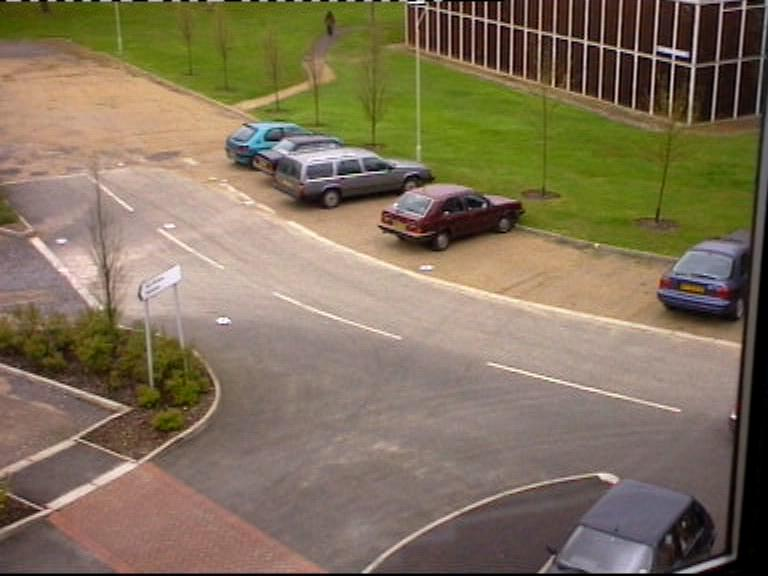
\includegraphics[width=0.2\linewidth]{fig2_a1} &
	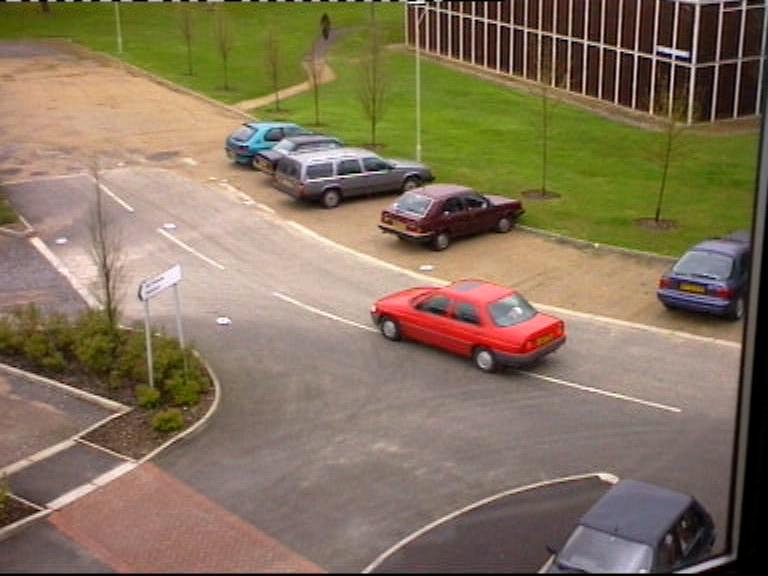
\includegraphics[width=0.2\linewidth]{fig2_b1} &
 	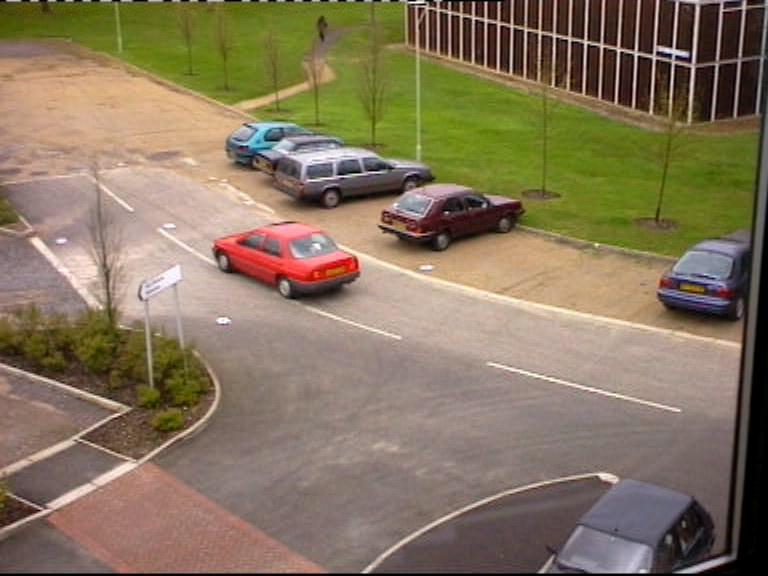
\includegraphics[width=0.2\linewidth]{fig2_c1} &
 	 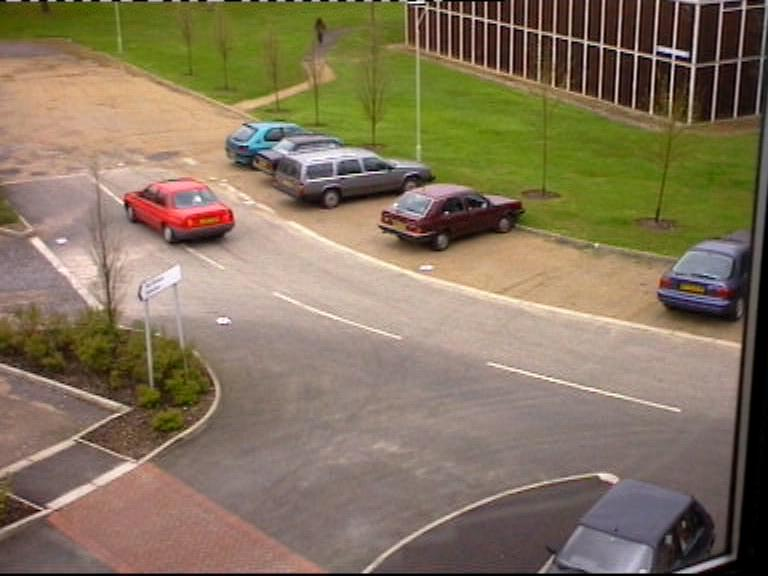
\includegraphics[width=0.2\linewidth]{fig2_d1} &
    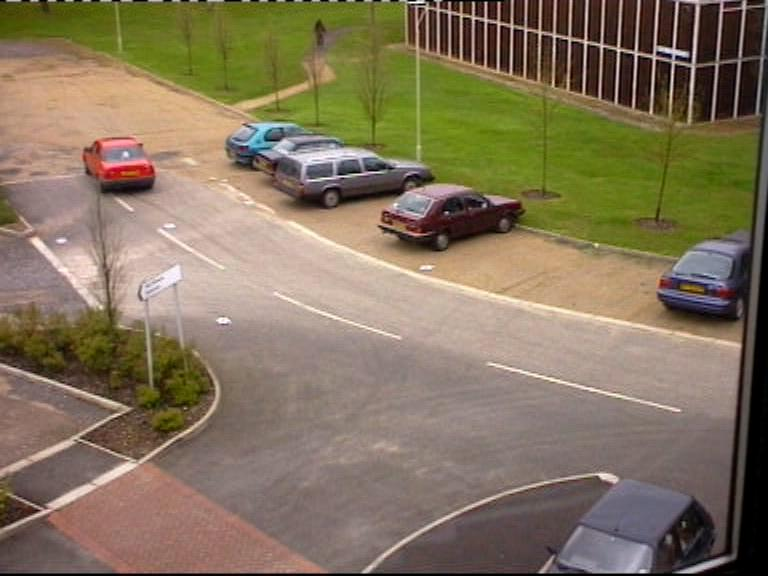
\includegraphics[width=0.2\linewidth]{fig2_e1} \vspace{-1mm}\\
	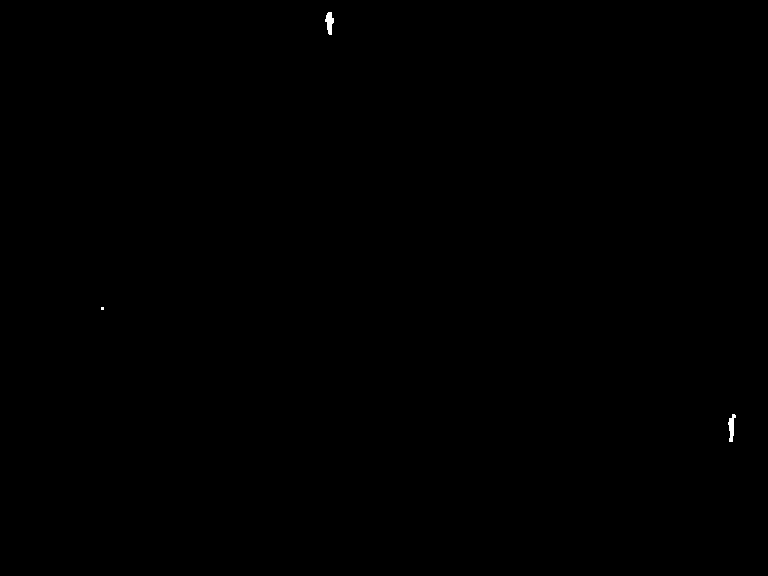
\includegraphics[width=0.2\linewidth]{fig2_a2} &
	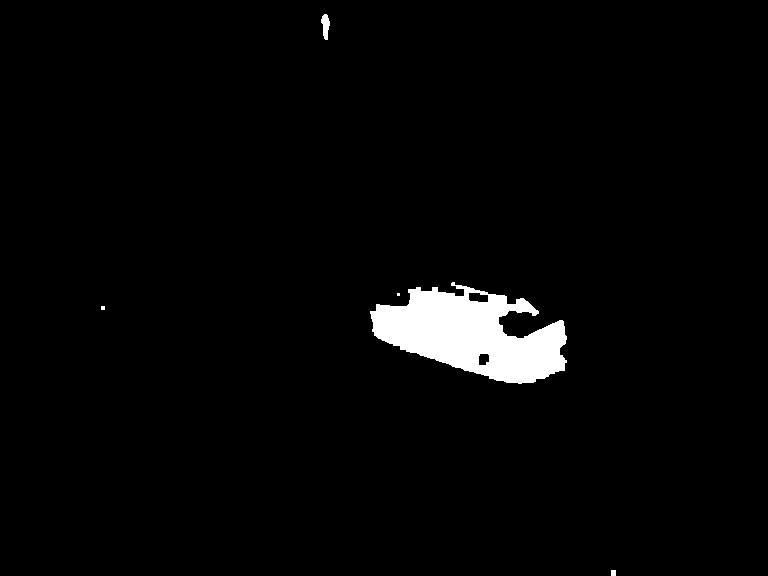
\includegraphics[width=0.2\linewidth]{fig2_b2} &
 	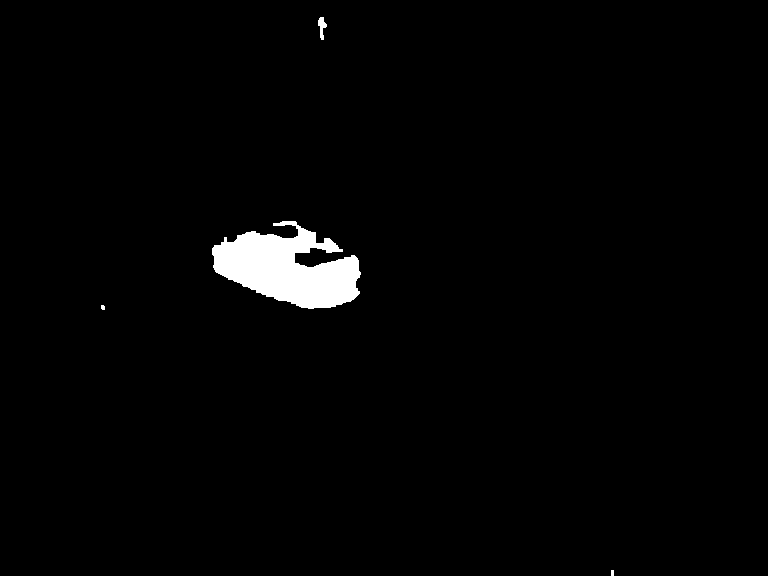
\includegraphics[width=0.2\linewidth]{fig2_c2} &
 	 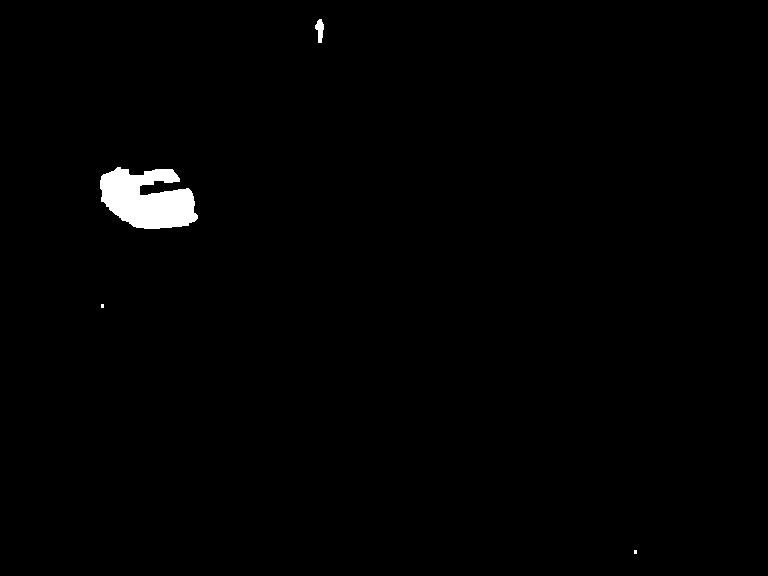
\includegraphics[width=0.2\linewidth]{fig2_d2} &
    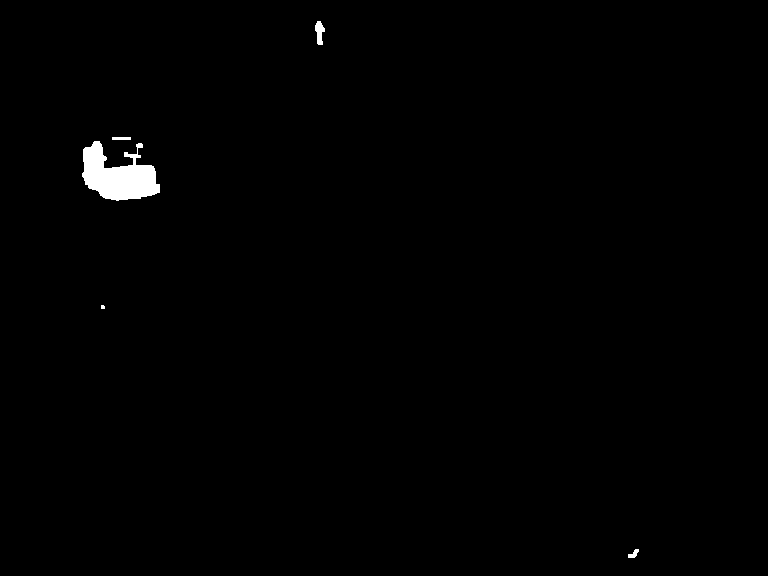
\includegraphics[width=0.2\linewidth]{fig2_e2} \vspace{-1mm}\\
    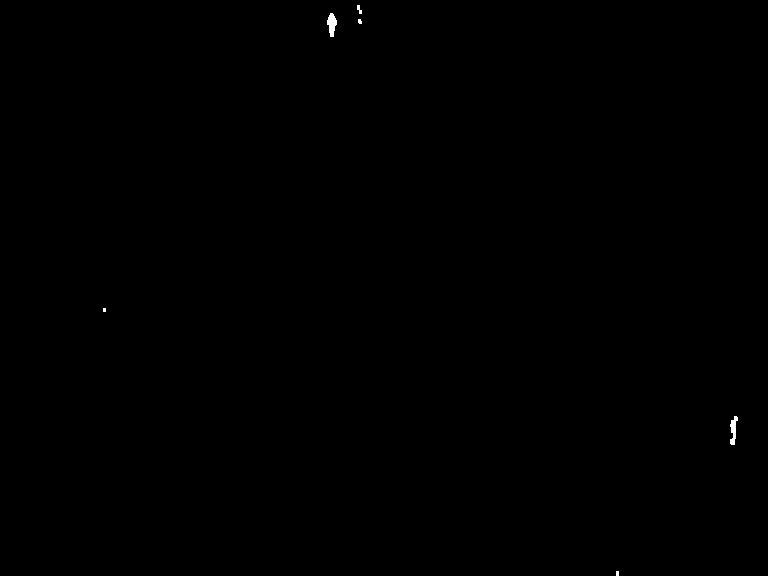
\includegraphics[width=0.2\linewidth]{fig2_a3} &
	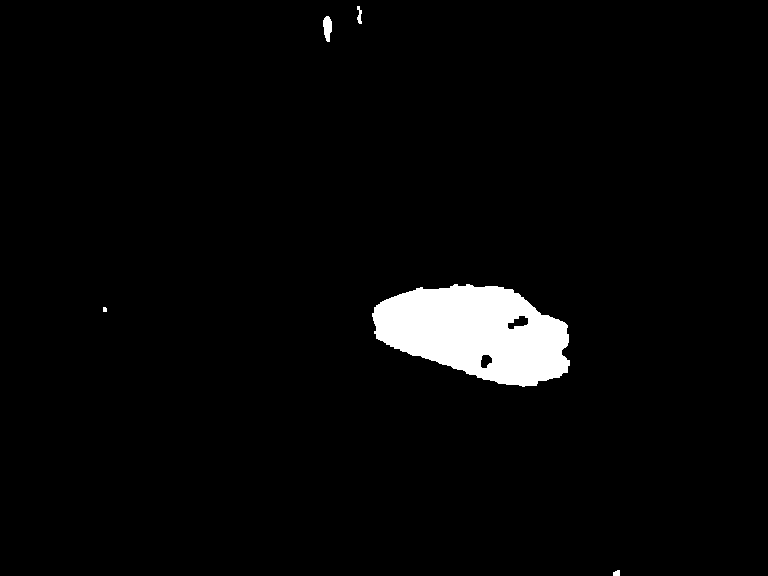
\includegraphics[width=0.2\linewidth]{fig2_b3} &
 	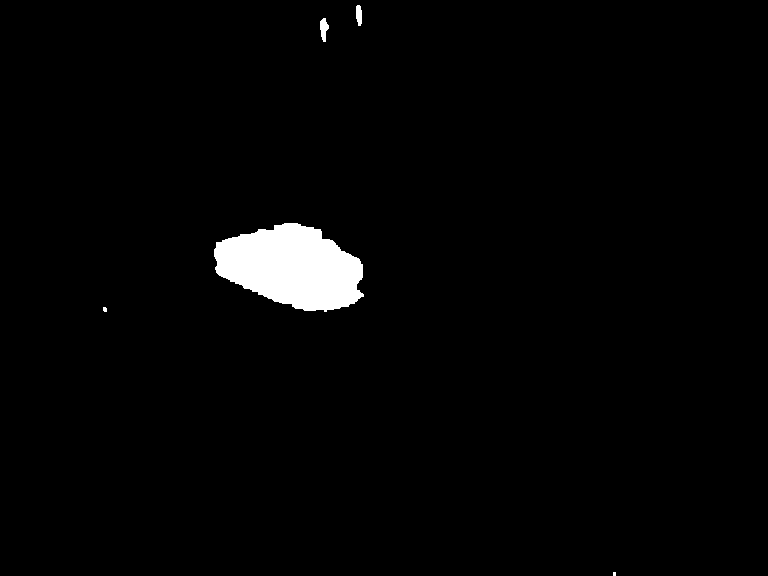
\includegraphics[width=0.2\linewidth]{fig2_c3} &
 	 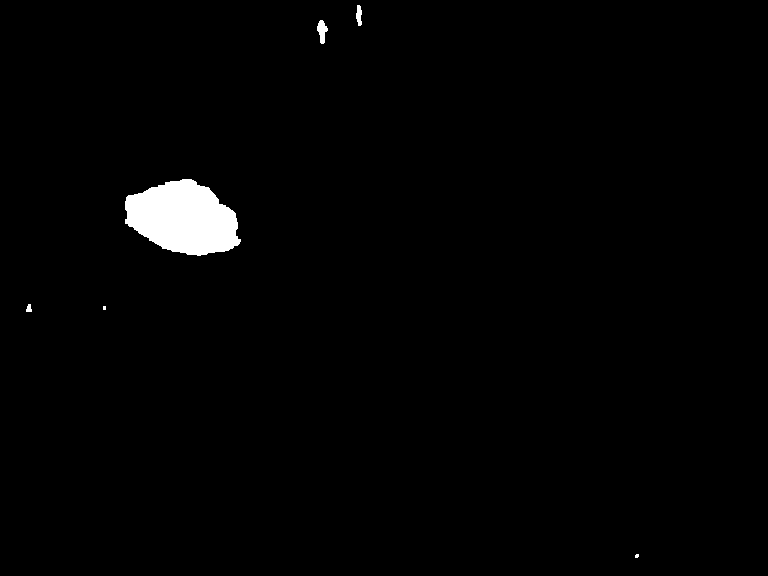
\includegraphics[width=0.2\linewidth]{fig2_d3} &
    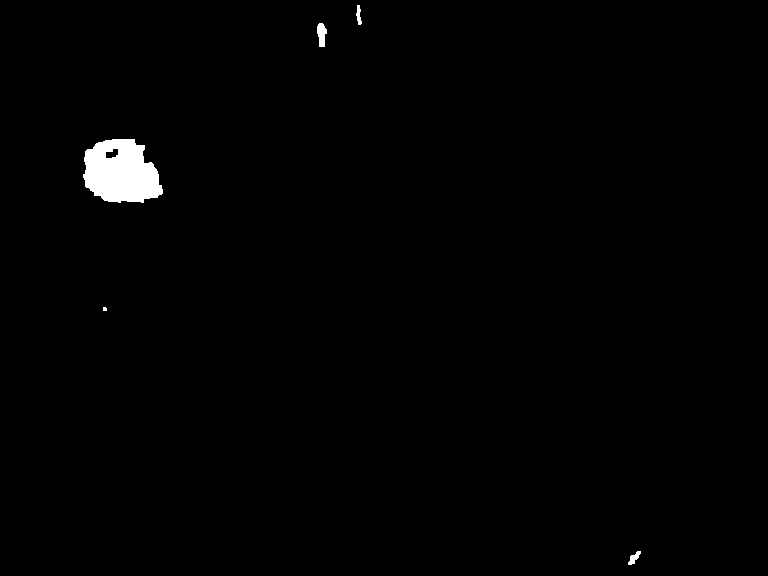
\includegraphics[width=0.2\linewidth]{fig2_e3} \vspace{-1mm}\\
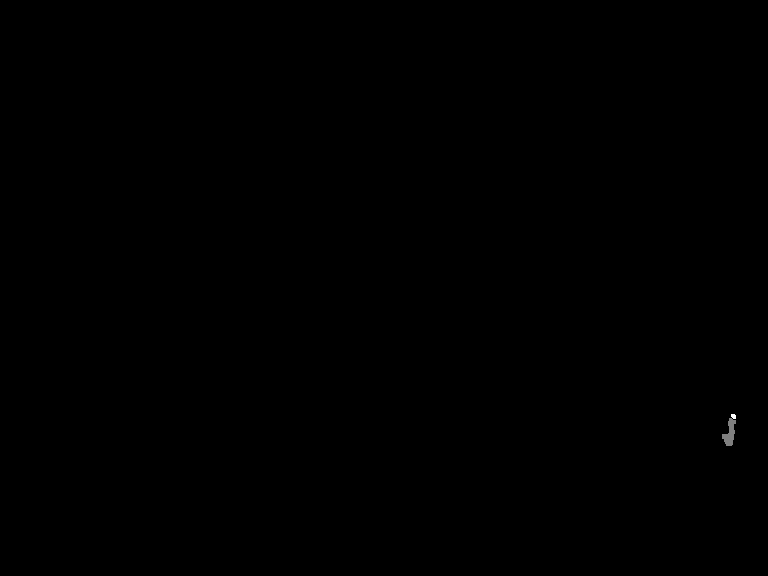
\includegraphics[width=0.2\linewidth]{fig2_a4} &
	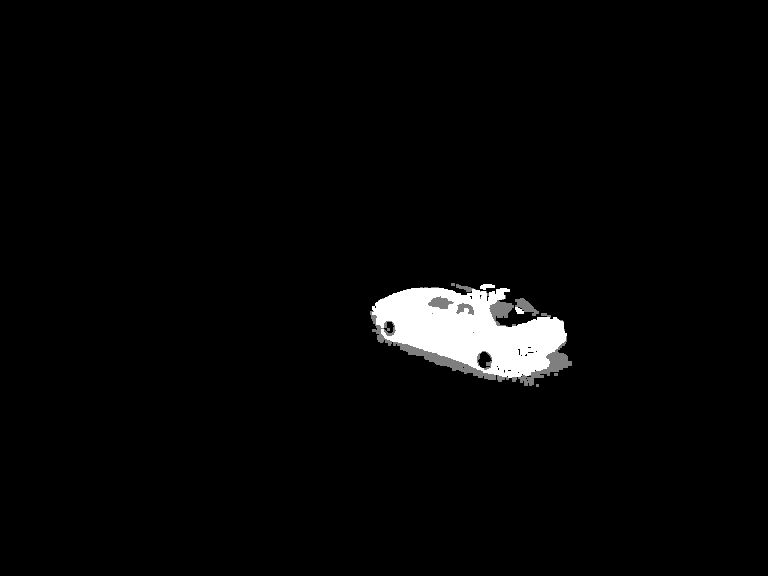
\includegraphics[width=0.2\linewidth]{fig2_b4} &
 	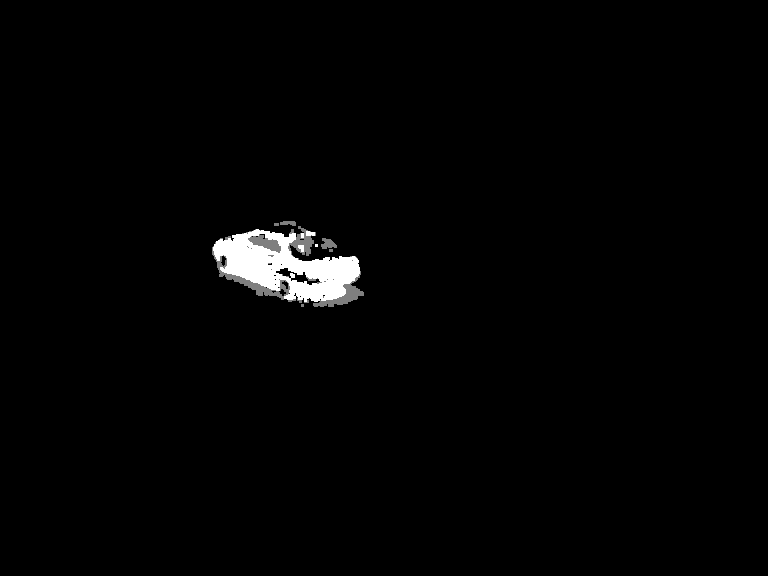
\includegraphics[width=0.2\linewidth]{fig2_c4} &
 	 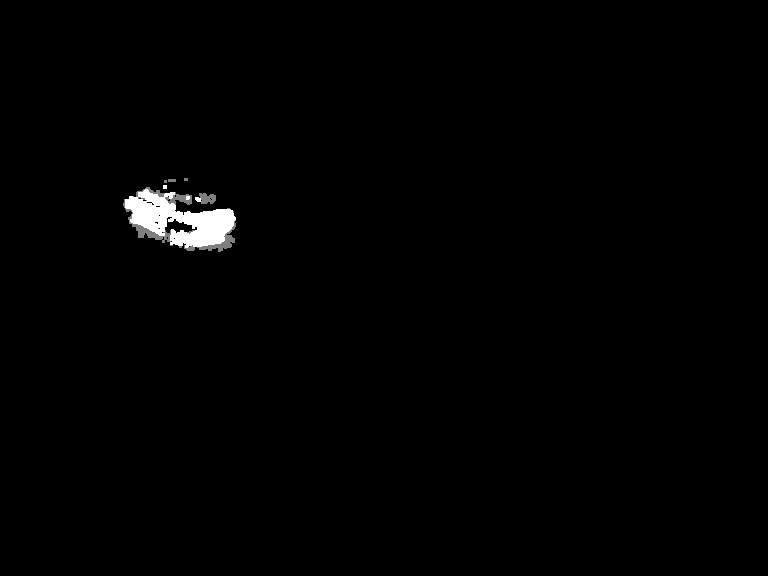
\includegraphics[width=0.2\linewidth]{fig2_d4} &
    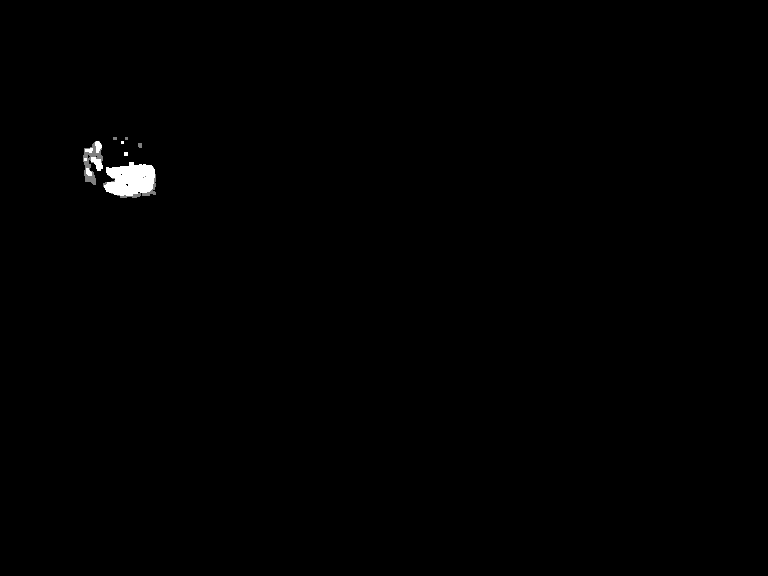
\includegraphics[width=0.2\linewidth]{fig2_e4} \vspace{-1mm}\\

    {\small (a)} &  {\small (b)}  &  {\small (c)} &  {\small (d)} \\
    \end{tabular}
	\captionof{figure}{\small 在 Scene\_Data 视频序列上实现混合高斯模型的背景建模。第一行:原始视频序列图像;第二行:手动实现的高斯混合模型;第三行: 分别在 R、G、B 三个通道手动实现的高斯混合模型;第四行:调用的 OpenCV 高斯混合模型函数。(a) 第一百一十帧, (b) 第一百三十五帧, (c) 第一百五十五帧, (d) 第一百七十五帧, and (e) 第二百帧.}
	\label{fig:result}
	\end{center}
	\vspace{0.5cm}
\end{minipage}
}]


\begin{figure}[!ht]
  \centering
  \begin{minipage}[b]{\linewidth} 
  \subfloat[]{
    \begin{minipage}[b]{0.18\linewidth} 
      \centering
      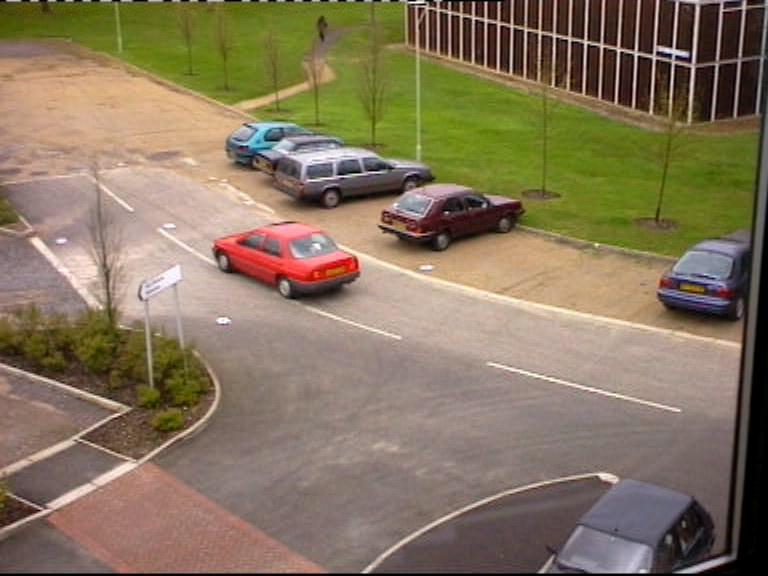
\includegraphics[width=\linewidth]{fig2_c1}
       \end{minipage}
  }
  \subfloat[]{
    \begin{minipage}[b]{0.18\linewidth} 
      \centering
      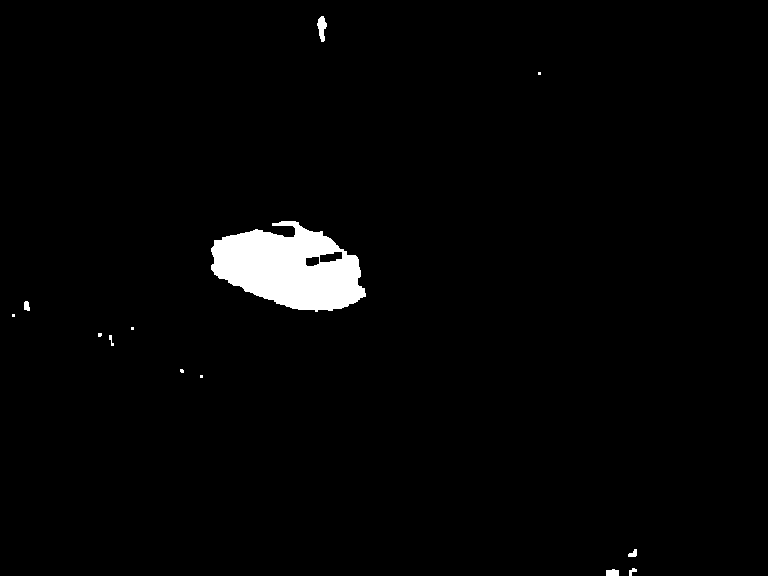
\includegraphics[width=\linewidth]{fig3_sigma20}
       \end{minipage}
  }
\subfloat[]{
    \begin{minipage}[b]{0.18\linewidth} 
      \centering
      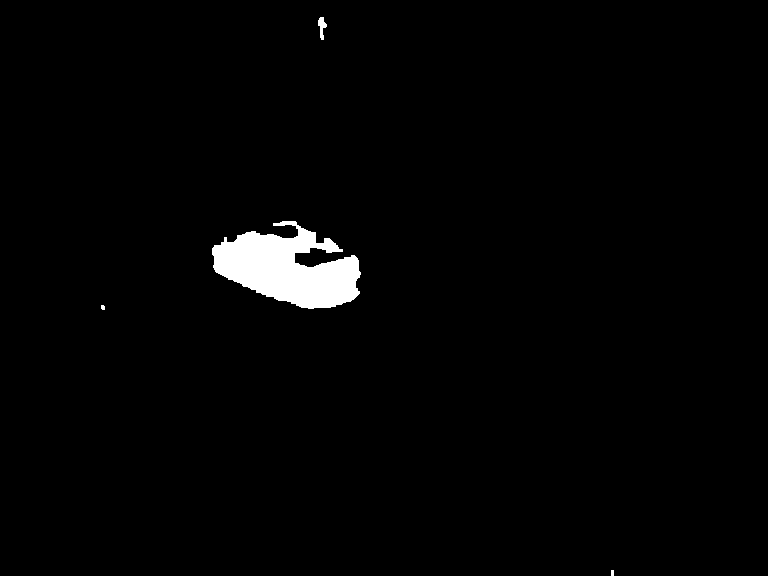
\includegraphics[width=\linewidth]{fig2_c2}
       \end{minipage}
  }
\subfloat[]{
    \begin{minipage}[b]{0.18\linewidth} 
      \centering
      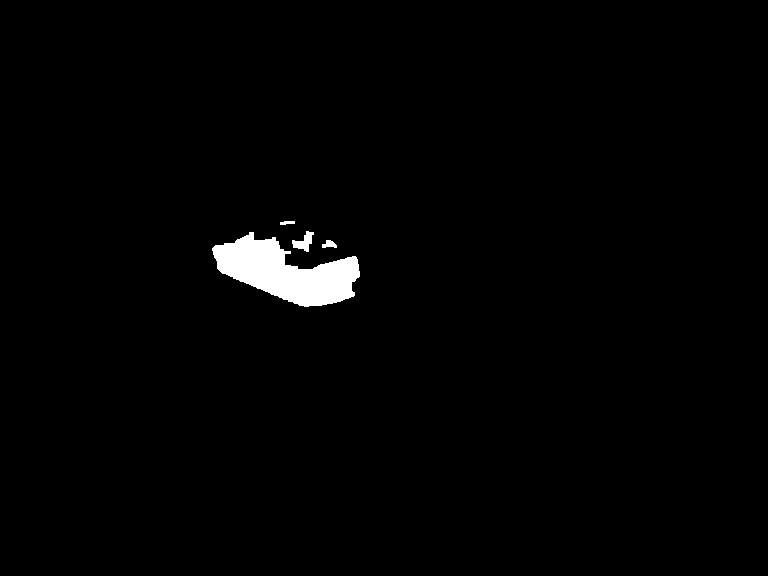
\includegraphics[width=\linewidth]{fig3_sigma50}
       \end{minipage}
  }
\subfloat[]{
    \begin{minipage}[b]{0.18\linewidth} 
      \centering
      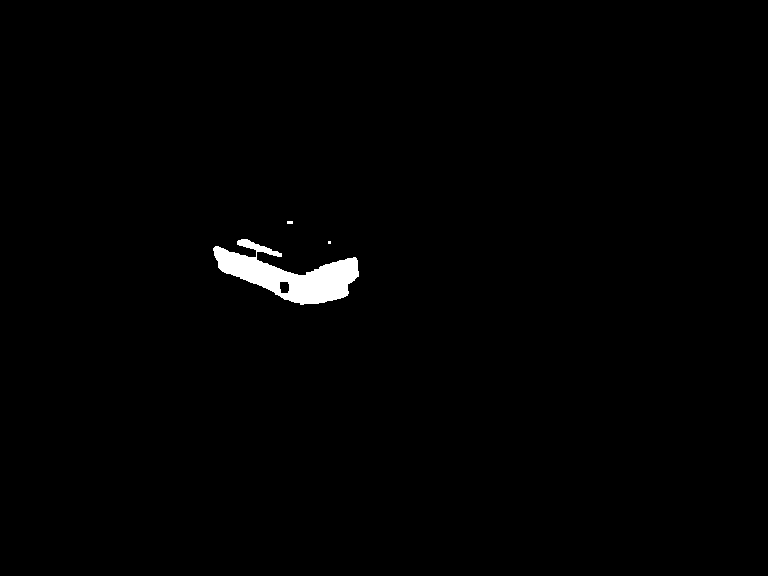
\includegraphics[width=\linewidth]{fig3_sigma80}
       \end{minipage}
  }

  \end{minipage}
  \vfill
  \caption{在 Scene\_Data 视频序列上实现实现混合高斯模型的背景建模: (a) 第一百五十五帧, (b) $\sigma=20$, (c) $\sigma=30$, (d) $\sigma=50$, and (e) $\sigma=80$, .}
  \label{fig:sigma}
\end{figure}

首先探讨参数 $\sigma$ 初始值对背景建模效果的影响,固定其他参数的取值,$\sigma$ 分别取 20、30、50 和 80,可视化结果如图 \ref{fig:sigma} 所示。可以看出,随着 $\sigma$ 的增大,视频序列图像中运动的物体被误分为背景的像素越多,即检测出的运动目标越来越不完整。其原因在于随着 $\sigma$ 的增大,允许像素值偏离均值的范围越大,从而前景被误分类符合背景像素某一高斯模型的可能性越大,最终导致其被误分为背景。同理,如果单高斯模型的权重初始值设置越小,则背景像素被当作前景的可能性也越大。

\begin{figure}[!ht]
  \centering
  \begin{minipage}[b]{\linewidth} 
  \subfloat[]{
    \begin{minipage}[b]{0.23\linewidth} 
      \centering
      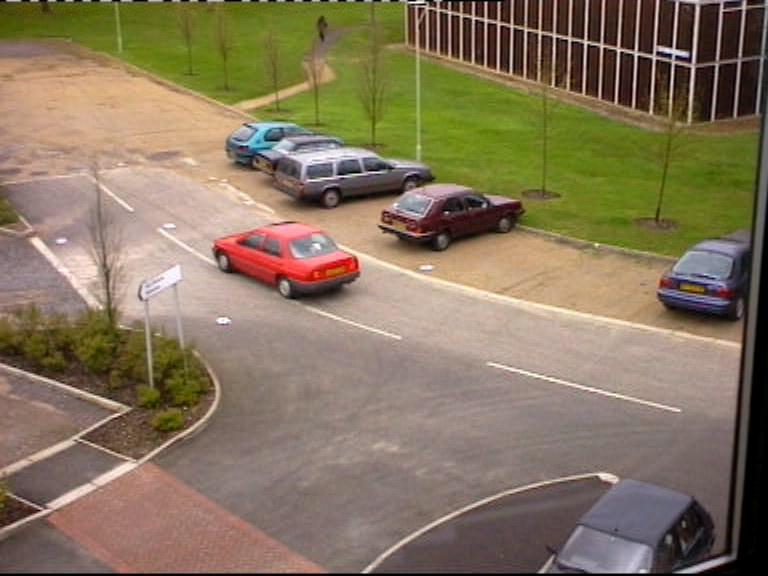
\includegraphics[width=\linewidth]{fig2_c1}
       \end{minipage}
  }
  \subfloat[]{
    \begin{minipage}[b]{0.23\linewidth} 
      \centering
      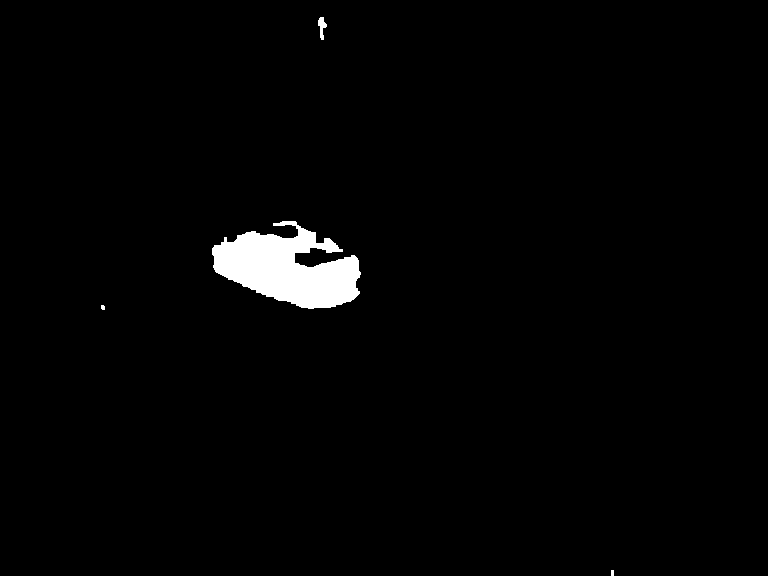
\includegraphics[width=\linewidth]{fig2_c2}
       \end{minipage}
  }
\subfloat[]{
    \begin{minipage}[b]{0.23\linewidth} 
      \centering
      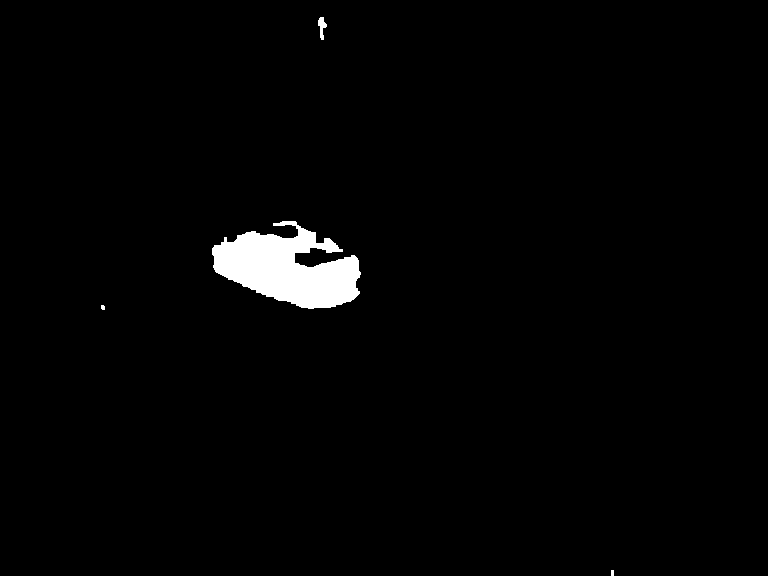
\includegraphics[width=\linewidth]{fig4_alpha001}
       \end{minipage}
  }
\subfloat[]{
    \begin{minipage}[b]{0.23\linewidth} 
      \centering
      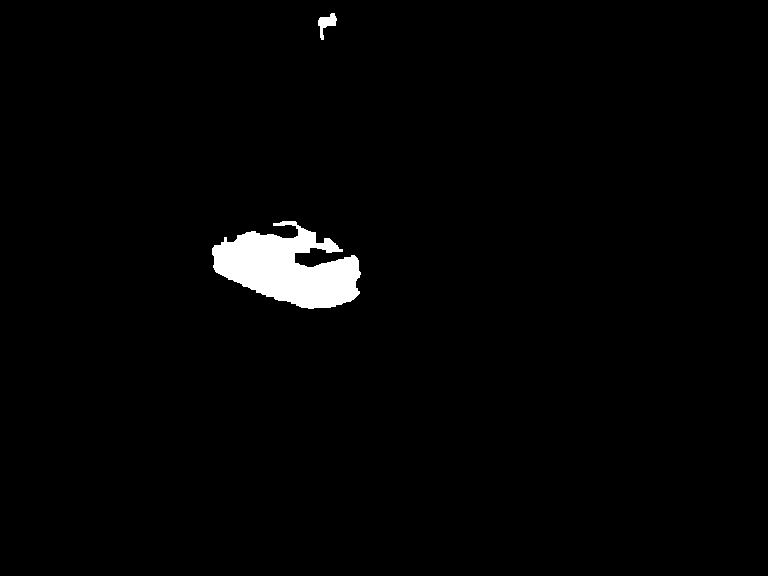
\includegraphics[width=\linewidth]{fig4_alpha01}
       \end{minipage}
  }

  \end{minipage}
  \vfill
  \caption{在 Scene\_Data 视频序列上实现实现混合高斯模型的背景建模: (a) 第一百五十五帧, (b) $alpha=0.005$, (c) $\alpha = 0.01$, and (c) $\alpha = 0.1$, .}
  \label{fig:alpha}
\end{figure}

其次,讨论参数 $\alpha$ 对背景建模效果的影响,固定其他参数的取值,$\alpha$ 分别取 0.005、0.01 和 0.1,可视化结果如图 \ref{fig:alpha} 所示。$\alpha$ 可以看作模型的“学习率”,可以看到模型在多帧训练的基础上,$\alpha$ 的取值对建模效果影响不大,略微在噪声和尺度较小的运动目标检测上有一定的区别。


